\chapter{Introduction}
\label{cha:introduction}

% \chapterquote{I'm awesome!}{Barney Stinson, WIRED magazine, 19.1.2009}

\section{Background}

As companies and consumers increasingly purchase goods online, the demand for cross carrier management platform
delivery services grows . Furthermore, the growth of online retail
sales has influenced the logistics industry for the past ten years and the trend is expected to
continue at least on a similar level during the next few years. 

\begin{figure}[!ht]
	\centering
	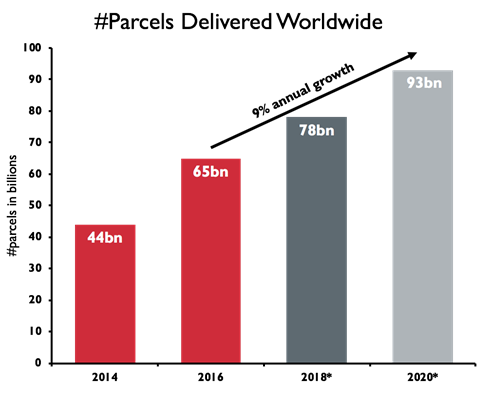
\includegraphics[width=0.5\textwidth]{images/ParcelsDel.png}\\
	\caption{Parcels Delivered worldwide [billions]}
	\label{fig:introduction__loremipsum}
\end{figure}

Responding to the increased demand of small-sized frequent shipments incurred by e-commerce has become one of the biggest challenges for logistics express delivery companies.
A successful delivery of shipments to consumers distributed across large geographical areas
will require re-designing of the existing system.

The increase of business-to-consumer (B2C) e-commerce activities implies that business are border less, global e-commerce is selling products or offer services across the world.


The idea to investigate delivery service based on the  blockchain proposed by the TU Berlin. The DC3 team in this project did not focus on implementing the blockchain system but rather in creating a platform interface to manage the parcel. At the end of the day, DC3 aims to be a part of a B2B blockchain solution that will make cross-border logistics much more reliable and efficient than they are now.   

Parcels are not always delivered at their destination in time and with the right agreed quality, this can cause financial losses due to reimbursements and low customer satisfaction. Especially higher value shipments ranging from routine parcels up to extraordinary parcels are insured against risks of loss, theft, damage or any other events that could impact delivery precision and quality. Prompt and secure detection, monitoring and recording of the shipment events is needed to allow tracking of service quality level, accountability, liability evidence in disputes and for analysis and optimization of the logistical chain.

DC3 (Dashboard for Control and Communication center) is a web-based dashboard for monitoring and controlling the logistics transactions beyond the border of a certain logistics company while leveraging DiLLaS (distributed ledger for logistics and supply chain management (DiLLaS). 

DiLLaS is an IoT and Blockchain solution that offers a new and unique view on shipment events data for logistics companies and their partners. These views create a detailed insight and transparency of significant security and safety events during the shipment. Additionally, by storing them in the distributed ledger, a trusted and decentralized recollection of the events of the shipment is created. DC3 enables a new way of handling parcel delivery and accelerates the implementation of more reliable and financial sustainable delivery processes.

The goal of DiLLaS is to provide a distributed ledger for the secure and trustworthy storage of events that occur during the transport of goods. A DiLLaS Mobile App will act as a client for the ledger and is intended as a means for all participants of a logistic chain to securely log a registration, deregistration and handover of a parcel within the distributed ledger. In combination with GRAVITY, the DiLLaS Mobile App will in addition be able to check the status of sensors that are attached to the parcels such temperature or humidity sensors and to log violations of predefined delivery conditions within the distributed ledger. Since DiLLaS makes use of Blockchain technology to persist the events and their related data in an immutable, transparent and a distributed manner where common incidents such as lost or delayed parcels can be securely traced back to its originators. With the commonly approved log of logistic events in DiLLaS, logistic operators will be able to improve their efficiency in terms of parcel delivery time by identifying bottle necks, costs per parcel by identifying unreliable partners and the quality of service by evaluating if parcels are delivered according to the predefined delivery conditions such as a constant temperature or an acceptable intensity of shocks for goods of high value. 


\section{Problem Discussion}

\subsection{Vendors communication and limitations}
There are multiple inefficiencies in cross-border delivery industry, related to lack of transparency and trust between the different logistics providers. International parcel delivery usually go through several logistics vendor, each on their side of the border, and there is a lot of accounting and interoperability overhead in the interactions between the different vendors. The idea is to solve these issues with the blockchain technology, taking advantage of its inherent transparency and trust.
From a Logistic company perspective, the parcel information is limited to their ownership and post completion of handover to a peer logistic company the package would not be efficiently tracked and the interrelated companies handling the package would not be in consensus. This common interface provides a plausible solution to the problem stated above by giving an opportunity for the companies to keep track of the package irrespective of the ownership of the package at a given point of time by having full information about it. It will also help the companies achieve better customer satisfaction by providing such sensor options to its customers to make use of.

\subsection{Vendors HMI}
From a customer perspective, when a customer orders a parcel the information revealed to him is depended on the quality of the carrier web interface, with a unique high-detailed dashboard the customer can be independent from the retail interface system and be informed about the status of the package and location of the package at all times throughout the journey of the package from source to destination.More options are made available to the customer in terms of a temperature and a shock sensor which is capable of taking lower and upper limits from the customer as an input and reverting with any irregularities in the package.




% \begin{table}[!ht]
% 	\small
% 	\centering
% 	\begin{tabular}{|l|l|l|l|}
% 		\hline
% 		Lorem & ipsum & dolor & sit \\
% 		\hline
% 		amet & consetetur & sadipscing & elitr \\
% 		\hline
% 		Lorem & ipsum & dolor & sit \\
% 		\hline
% 		amet & consetetur & sadipscing & elitr \\
% 		\hline
% 	\end{tabular}
% 	\caption{Lorem ipsum...}
% \end{table}


% \subsubsection{Even more Lorem Ipsii}

% alon